\chapter{En god begynnelse}
\section{Våre første små tester: print, Spyder}
\todo[author=Christian]{Heading uten brødtekst...fy...}
\subsection*{Først litt om Spyder}
\begin{figure}[h]
\begin{center}
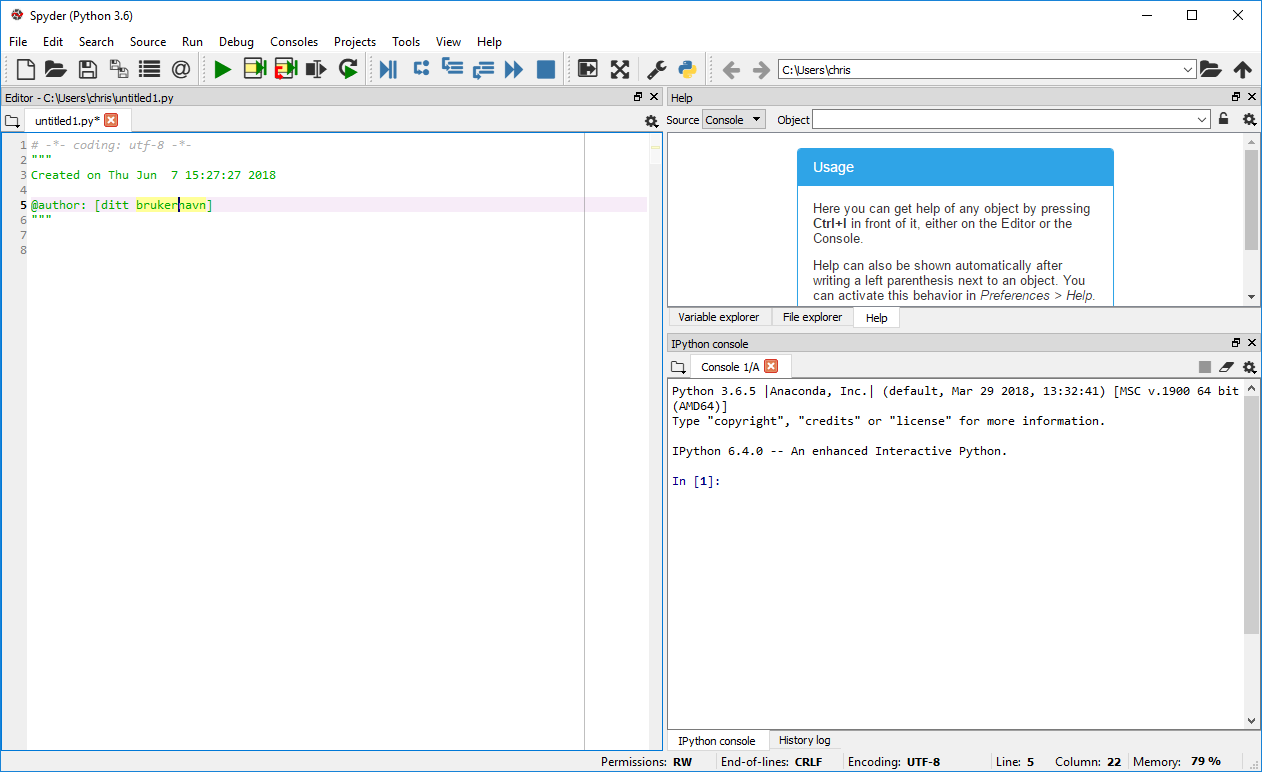
\includegraphics[width=1.0\textwidth]{img/spyder_overview.png}
\end{center}
\caption{Spyder}
\label{fig:spyder_overview}
\end{figure}

\todo[author=christian]{Trenger kanskje ikke så mye tekst siden vi har fått inn bilde}
Start Spyder. Du skal da på skjermen ha et stort vindu, typisk med tittel Spyder (Python 3.6) Helt øverst er den vanlige menylinjen (File Edit Search ... Projects ...) etc. Like under er der en linje med div. ikoner. Dette er ulike toolbars. De er snarveier til funksjonaliteter som også kan nås fra menylinjen. Toolbarene kan flyttes rundt eller fjernes helt ved View / Toolbars / og klikke de av.) Vi trenger ikke tenke på disse ennå. 

Under linjen med toolbars, på venstreside har du Editor-vinduet. Det er et tekstbehandlingsprogram.  Her er det du skriver inn python-programmet ditt, linje for linje. Du kan flytte deg rundt med piltastene (og musen). (Ikke skriv noe ennå.) 

Hvis dette er første gangen du bruker Spyder, vil Spyder ha lagt inn noe tekst i et nytt dokument (program/fil). På linje 5 eller 6 vil det stå @author og brukernavnet ditt. Navnet på filen står øverst, noe slikt som untitled1.py. Dette er en fil som spyder har åpnet og som ikke gjør noe ennå. Hvis du allerede har brukt Spyder litt, vil kanskje den siste fil/programmet du arbeidet med være i editoren.

Når programmet (det du har skrevet inn) er passe klart, kjører (eksekverer, execute) du det ved å trykke på den grønne "play"-knappen, like under menylinja øverst. (Den viser "Run file (F5)" når du tar musepekeren over knappen). Ikke gjør det nå. Vi skal ikke bruke editoren nå helt i begynnelsen.

På høyresiden, nederst, har du Python/IPython-vinduet, også kalt konsollen (Console). Nederst står det \todo[author=Christian]{Det ser ikke ut som det er default at Python consolen vises lenger} Python console, IPython console og kanskje History log. Klikk på flappen med IPython console. (Du kan også bruke Python console, men IPython er å foretrekke.) I IPython-vinduet kan du skrive python-kommandoer direkte inn. Det skal vi gjøre mye av nå i begynnelsen. (I'en i IPython står for interaktivt, dvs. to-veis kommunikasjon mellom deg og python.) 

På høyresiden, over IPython-konsollen er der et vindu. Dette har flapper Help, Variable explorer og File explorer. Litt mer om det nedenfor. 

Python har mange kommandoer (funksjoner) innebygd. Det er disse vi bruker når vi programmerer. Den første funksjonen vi trenger er print (skriv til skjerm), Klikk på (inne i) IPython-vinduet for å aktivere det. Skriv så første linja nedenfor og trykk ENTER:
\begin{lstlisting}[caption={Din første Python kode}]
print(365)
\end{lstlisting}
Python skriver ut 365.

Prøv:
\begin{lstlisting}[caption={Din andre Python kode}]
print("Hei Python")
\end{lstlisting}

(Merk at tekst må stå innenfor hermetegn)

print() er en funksjon, og funksjoner tar argumenter i parentes. Argumentet til print er det som skal printes, her tekststrengen ``Hei Python'' eller tallet 365. 

\subsubsection{Variabler}
En variabel er noe som inneholder en verdi. En variabel har et navn og en verdi.

\begin{lstlisting}
min_var1 = "Hei Python!"
\end{lstlisting}

Navnet er \lstinline{min_var1}, verdien er ``Hei Python''. Det er en tekststreng (str). 

\begin{lstlisting}
min_var2 = 365
\end{lstlisting}

Navnet er \lstinline{min_var2}, verdien er 365, det er et (hel)tall (int). 

\begin{lstlisting}
min_var2 = 300
\end{lstlisting}

Nå skiftet vi verdi. 

Du kan godt ha mellomrom, linjene over kan også skrives som: 
\begin{lstlisting}
min_var2=300
min_var2= 300
min_var2 =300
\end{lstlisting}

Men du kan ikke skrive \lstinline{min var2 = 300} for variabelen heter \lstinline{min_var2}, den må være i ett ord. 

Nå kan vi printe variabelen:
\begin{lstlisting}
print(min_var1)
\end{lstlisting}
Flere variabler og verdier kan printes samtidig:
\begin{lstlisting}
print(min_var1, "Det er", min_var2, "dager i et år.")
\end{lstlisting}

I IPython-vinduet kan du bruke piltastene for å hente frem igjen det du har skrevet tidligere. Prøv pil opp. Og ned igjen. Du kan endre på linja. Trykk ENTER for å kjøre/utføre (eksekvere) linja (på nytt). (Eller visk ut linja eller trykk piltast ned til du får tom linje.) Du kan også se alt du har skrevet i vinduet ved å trykke på History log nederst. (Gå tilbake til IPython-vinduet.) 

\subsection{Variable explorer}

Nå har du definert et par variabler (min\_{}var1 og min\_{}var2). I vinduet oppe til høyre, kan du se innholdet til variablene. Klikk på flappen ``Variable explorer''. Det kan være nyttig når du har litt større programmer og programmet ikke helt oppfører seg som du tenkte. (Mer om debugging senere.) 

I IPython-vinduet trenger du forsåvidt ikke bruke print for å se verdien til en variabel, bare skriv navnet og trykk ENTER:
\begin{lstlisting}
min_var1
\end{lstlisting}

Det blir ikke helt som med print. Hermetegnene vises. Og det er dessuten enkle hermetegn, og ikke doble som vi brukte. Både doble og enkle hermetegn kan brukes i Python. Men de må stemme parvis. Du kan ikke skrive:

\begin{lstlisting}
min\_{}var3 = 'Hei"
\end{lstlisting}

Da får du en feilmelding: ``SyntaxError''

\subsection{Feilmeldinger}

Når du skriver noe som python ikke forstår, får du en feilmelding.  Lag noen feil og se hva Python svarer:

\iffalse

asdf
Du får NameError - python aner ikke hva asdf skal bety 
'asdf'
Nå er asdf innenfor hermetegn, og da er det bare en verdi. Python klager ikke.
a = "asdf
SyntaxError: EOL while scanning string literal

Du vil komme borti flere feilmeldingerstyper. 
Det er viktig å skjønne hva feilmeldingen betyr.  
I interaktiv kjøring, er det alltid siste kommando som er feil, så vi vet hvor feilen er. 
Når vi kjører et program fra fil, og noe går galt, forteller Python i hvilken linje
feilen oppstod. Det er praktisk. 


TAB-COMPLETION: 
IPython-vinduet ditt kan hjelpe deg med å skrive raskere.
F.eks. skriv pri og trykk TAB. IPython fullfører så med å legge til nt så det blir print.
Det er den i stand til fordi der kun er én kommando som begynner med pri.
Dersom du bare skriver pr og trykker TAB kommer det opp noen flere alternativer.
Du kan velge med piltastene (og ENTER eller TAB), eller trykke Escape (ESC) for å kansellere.

TAB-completion plukker også opp variabler.
Dersom du skriver mi og trykker TAB, blir en n lagt til så du har min,
og du får flere alternativ, min (som er en funksjon som vi skal komme tilbake til),
eller variablene du selv har definert, min_var1, min_var2 og min_var3.






SPYDER
Restarte IPython-vinduet.
Noen ganger henger IPython-vinduet, og du må restarte for å komme videre.
Eller du har kanskje lyst til å bli kvitt alle variablene du har definert,
starte med blanke ark. 
Da kan du trykke på Consoles i hovedmenyen øverst, deretter Restart kernel. 
Da går det noen sekunder, så kommer et nytt, rent IPython-vindu opp.
(NB: du mister altså alle variablene du har laget.) 
(Du trenger ikke gjøre det nå.)

Du kan også ha flere IPython- og/eller Python-terminaler oppe samtidig.
Klikk Consoles, og deretter 
Open an IPython console
eller 
Open a Python console


Restarte Spyder.
Dersom du vil ta ned hele Spyder: Se oppe til venstre, trykk File, så Quit. 
(Ikke gjør det nå.) 


Litt mer om Spyder: Layout 
Spyder er en GUI (Grafisk User Interface, grafisk brukergrensesnitt)
som gjør det enklere å arbeide med Python.
Spyder eksisterer for windows/mac/linux og er open source og gratis. 
Vi har installert det som en del av Anaconda eller Miniconda. 
(Det går naturligvis også an å kjøre Python uten Spyder.)


Spyder har mange funksjonaliteter.
(Se de mange valgene i hovedmenyen øverst i vinduet.)
En av disse er hvordan layouten skal være. 
Trykk på View / Window layouts.
Sansynligvis er det Spyder Default Layout du bruker.
Du kan velge en av de andre, f.eks. Matlab Layout.
Den gir deg flere vinduer med informasjon, som kan være nyttig.
Men vi holder oss til Spyder Default Layout.

Du kan justere størrelsen på vinduene med musen. 

Du kan øke/minske tekststørrelsen i Editor-vinduet og IPython-terminal-vinduet
(uavhengig av hverandre) med CTRL+ / CTRL- mens vinduet er aktivt. 

Noe som kan være praktisk nå i begynnelsen, er muligheten til å lagre alt
som er gjort i IPython-vinduet. 
Aktiver IPython-vinduet. Trykk så CTRL+s (CTRL og s).
Da kommer et vindu opp som lar deg lagre IPython-aktiviteten som html-fil.
Velg et passende navn (og katalog).
Filen må leses med en nettleser (Firefox, IE/Edge, Safari).
(Enten kan du finne filen med f.eks. Windows Explorer, dernest klikke på den. 
Eller du kan åpne en ny tab/vindu i nettleseren og skrive file:/// i url-en.
Da vil du få opp filstrukturen din. Du må da klikke deg frem til rett sted og finne filen.)
Det går imidlertid ikke an å laste det inn igjen i spyder og slik fortsette der du slapp. 


Oppgave 1:
Bruk et minutt eller to på å gjøre deg litt kjent med Spyder.
Endre litt på vindusstørrelse, klikke på ulike flapper, sjekke hva menyene inneholder. 

Oppgave 2:
Lag to variabler som inneholder tall. Lag to variabler som inneholder tekst.
Skriv ut innholdet av de fire variablene. Se om de er i Variable explorer-vinduet.
Endre innholdet til en av variablene. Se om variabelverdien endres i Variable explorer.

Oppgave 3:
Lagre en html-fil med IPython-aktiviteten din og finn den igjen med en nettleser. 


REF: For mer Spyder-info: klikk på Help-flappen på vinduet øverst til høyre
(som også har flappen Variable explorer).
Der kan du ved anledning (senere) følge en tutorial (klikk tutorial)
som beskriver ganske greit hva Spyder har å tilby.


\fi